
\chapter{Advanced Algebra – Functions, Graphs, and Equations}

\section{Introduction: The Power of Algebra in Solving Real-World Problems}
Now that you’ve built a strong foundation in basic algebra, we’re ready to explore advanced algebra concepts, such as functions, equations, and graphs. Algebra is about identifying and understanding relationships between numbers, but when those relationships get more complex, we need new tools to make sense of them. That’s where functions and graphs come in.

In this chapter, you’ll learn how to work with different types of equations, understand the concept of functions, and graph relationships between variables. These skills will help you solve more complex problems and visualize how numbers relate to each other.

\section{What Is a Function?}
A function is a rule that assigns exactly one output (result) for each input. You can think of it like a machine: You put in an input (like a number), the function processes it, and you get an output.

Functions are written like this:
\[ f(x) = 2x + 3 \]

In this function:
\begin{itemize}
    \item \( x \) is the input (the number you put in).
    \item \( f(x) \) is the output (what you get after applying the function rule).
    \item The rule is to multiply \( x \) by 2 and then add 3.
\end{itemize}

Example: If \( x = 4 \), then:
\[ f(4) = 2(4) + 3 = 8 + 3 = 11 \]
So, the output is 11 when the input is 4.

Another Example: If \( x = -2 \), then:
\[ f(-2) = 2(-2) + 3 = -4 + 3 = -1 \]

\section{Line Graphs}

A line graph visually represents a function, showing how the output changes with varying input. It helps identify patterns and relationships between variables.

\subsection{Graphing Linear Functions}

To graph a linear function \( f(x) = mx + b \):

\begin{enumerate}
    \item Identify the slope (\( m \)) and y-intercept (\( b \)).
    \item Plot the y-intercept at point \((0, b)\).
    \item Use the slope to determine another point: from \((0, b)\), move right 1 unit and up or down by \( m \).
    \item Draw a straight line through the points.
\end{enumerate}

\textbf{Example:} Graph \( f(x) = -\frac{1}{2}x + 3 \).

\begin{itemize}
    \item \( b = 3 \), so plot \((0, 3)\).
    \item \( m = -\frac{1}{2} \): for every 1 unit right, move 0.5 units down. Plot \((2, 2)\).
    \item Connect the points with a line.
\end{itemize}

\section{Linear Functions}

A linear function forms a straight line and follows:

\[
f(x) = mx + b
\]

Where:
\begin{itemize}
    \item \( m \): slope (how steep the line is)
    \item \( b \): y-intercept (where the line crosses the y-axis)
\end{itemize}

\textbf{Example:} \( f(x) = 2x + 1 \).

\begin{itemize}
    \item \( m = 2 \), meaning for each 1 unit increase in \( x \), \( f(x) \) increases by 2.
    \item \( b = 1 \), so the line crosses at \((0, 1)\).
\end{itemize}

To graph:

\begin{enumerate}
    \item Plot \( (0, 1) \).
    \item From \((0, 1)\), use the slope to plot \((1, 3)\).
    \item Draw a straight line through the points.
\end{enumerate}


\section{Solving Linear Equations}
A linear equation is an equation that makes a straight line when graphed. Solving a linear equation means finding the value of the variable (usually \( x \)) that makes the equation true.

Example: Solve \( 3x + 4 = 13 \).
\begin{enumerate}
    \item Subtract 4 from both sides:
    \[ 3x = 9 \]
    \item Divide both sides by 3:
    \[ x = 3 \]
\end{enumerate}
The solution is \( x = 3 \).

\section{Quadratic Functions}

A quadratic function is more complex than a linear function and has the form:
\[
f(x) = ax^2 + bx + c
\]

Where \( a \), \( b \), and \( c \) are constants. In contrast to linear functions, which graph as straight lines, the graph of a quadratic function is a curve called a parabola.

\begin{itemize}
    \item If \( a > 0 \), the parabola opens \textbf{upward}.
    \item If \( a < 0 \), the parabola opens \textbf{downward}.
\end{itemize}

\textbf{Example:} Consider the quadratic function:
\[
f(x) = x^2 - 4x + 3
\]

\begin{figure}[h!]
    \centering
    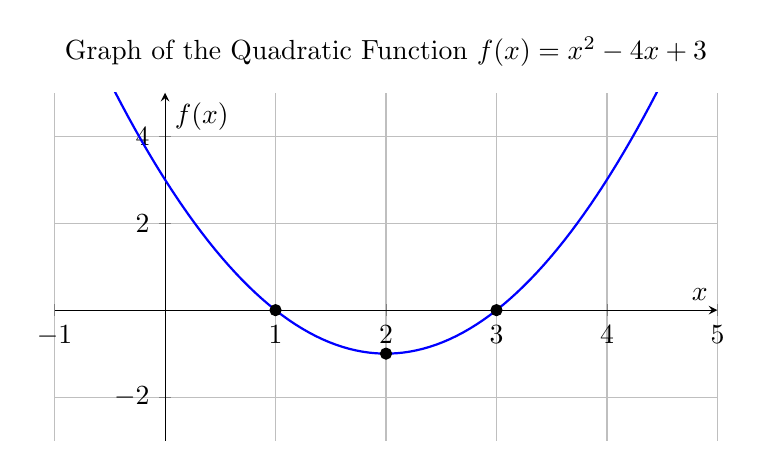
\begin{tikzpicture}
        \begin{axis}[
            axis lines = middle,
            xlabel = \(x\),
            ylabel = {\(f(x)\)},
            ymin=-3, ymax=5,
            xmin=-1, xmax=5,
            grid = major,
            width=10cm,
            height=6cm,
            domain=-1:5,
            samples=100,
            title={Graph of the Quadratic Function \( f(x) = x^2 - 4x + 3 \)}
        ]
        \addplot[blue, thick] {x^2 - 4*x + 3};
        \addplot[only marks, mark=*] coordinates {(2,-1) (1,0) (3,0)};
        \end{axis}
    \end{tikzpicture}
    \caption{The graph of the quadratic function \( f(x) = x^2 - 4x + 3 \). It shows the vertex, axis of symmetry, and additional points.}
\end{figure}

\subsection{Graphing a Quadratic Function}

The process of graphing a quadratic function involves several steps, which help illustrate the function's behavior and its differences from linear functions.

\begin{enumerate}
    \item \textbf{Find the Vertex:}
    \begin{itemize}
        \item The vertex represents the highest or lowest point of the parabola, depending on whether it opens upward or downward.
        \item Use the formula for the x-coordinate of the vertex:
        \[
        x = -\frac{b}{2a}
        \]
        \item Substitute this value of \( x \) into the function \( f(x) \) to find the y-coordinate of the vertex:
        \[
        y = f\left( -\frac{b}{2a} \right)
        \]
        \item The vertex is at the point \(\left( -\frac{b}{2a}, f\left( -\frac{b}{2a} \right) \right)\).
    \end{itemize}
    
    \item \textbf{Determine Whether the Parabola Opens Upward or Downward:}
    \begin{itemize}
        \item If \( a > 0 \), the parabola opens upward, and the vertex is the minimum point.
        \item If \( a < 0 \), the parabola opens downward, and the vertex is the maximum point.
    \end{itemize}
    
    \item \textbf{Plot the Vertex:}
    \begin{itemize}
        \item Plot the vertex on the graph.
    \end{itemize}
    
    \item \textbf{Find the Axis of Symmetry:}
    \begin{itemize}
        \item The axis of symmetry is the vertical line passing through the vertex, which divides the parabola into two mirror images.
        \item The equation of the axis of symmetry is:
        \[
        x = -\frac{b}{2a}
        \]
    \end{itemize}
    
    \item \textbf{Plot Additional Points:}
    \begin{itemize}
        \item Choose x-values to the left and right of the vertex to find additional points on the parabola.
        \item Substitute these x-values into the function to calculate the corresponding y-values.
        \item Plot these points on the graph.
        \item Due to symmetry about the axis of symmetry, points on one side of the vertex will have corresponding points on the opposite side.
    \end{itemize}
    
    \item \textbf{Draw the Parabola:}
    \begin{itemize}
        \item Connect the vertex and all additional points with a smooth curve to create the parabola.
        \item Make sure the curve passes through all plotted points and extends infinitely in both directions.
    \end{itemize}
\end{enumerate}

\subsection{Example: Graphing the Quadratic Function \( f(x) = x^2 - 4x + 3 \)}

Let's apply the steps to graph \( f(x) = x^2 - 4x + 3 \).

\begin{itemize}
    \item \textbf{Find the Vertex:}
    \begin{enumerate}[label=(\alph*)]
        \item \( a = 1 \), \( b = -4 \), \( c = 3 \).
        \item Find the x-coordinate of the vertex:
        \[
        x = -\frac{-4}{2 \times 1} = 2
        \]
        \item Find the y-coordinate by substituting \( x = 2 \) into \( f(x) \):
        \[
        y = (2)^2 - 4(2) + 3 = -1
        \]
        \item The vertex is at \( (2, -1) \).
    \end{enumerate}
    
    \item \textbf{Axis of Symmetry:} \( x = 2 \).
    
    \item \textbf{Plot Additional Points:}
    \begin{enumerate}[label=(\alph*)]
        \item Choose values for \( x \), such as \( x = 1 \) and \( x = 3 \).
        \item When \( x = 1 \):
        \[
        f(1) = 1^2 - 4(1) + 3 = 0
        \]
        Plot the point \( (1, 0) \).
        \item When \( x = 3 \):
        \[
        f(3) = 3^2 - 4(3) + 3 = 0
        \]
        Plot the point \( (3, 0) \).
    \end{enumerate}
    
    \item \textbf{Draw the Parabola:} Connect the vertex and the points \( (1, 0) \), \( (3, 0) \) with a smooth curve.
\end{itemize}

\begin{figure}[h!]
    \centering
    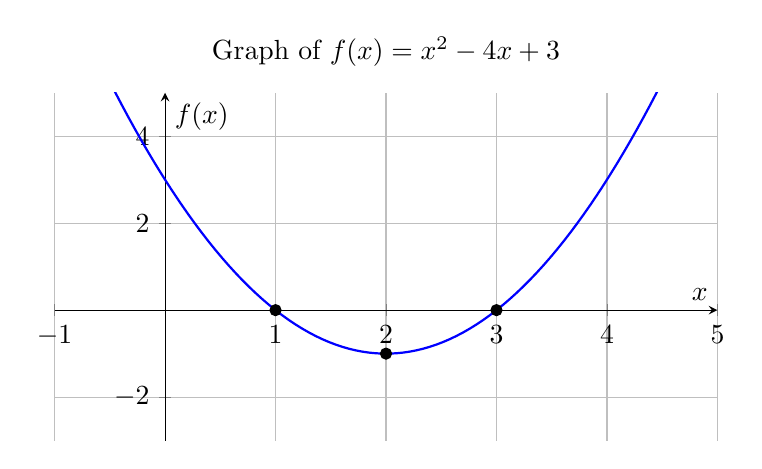
\begin{tikzpicture}
        \begin{axis}[
            axis lines = middle,
            xlabel = \(x\),
            ylabel = {\(f(x)\)},
            ymin=-3, ymax=5,
            xmin=-1, xmax=5,
            grid = major,
            width=10cm,
            height=6cm,
            domain=-1:5,
            samples=100,
            title={Graph of \( f(x) = x^2 - 4x + 3 \)}
        ]
        \addplot[blue, thick] {x^2 - 4*x + 3};
        \addplot[only marks, mark=*] coordinates {(2,-1) (1,0) (3,0)};
        \end{axis}
    \end{tikzpicture}
    \caption{Graph of the quadratic function \( f(x) = x^2 - 4x + 3 \) showing the vertex, axis of symmetry, and additional points.}
\end{figure}

\subsection{Connecting Quadratic Functions to Linear Functions}

Quadratic functions and linear functions differ significantly in their graphical representation and behavior:

\begin{itemize}
    \item \textbf{Linear functions} graph as straight lines, indicating constant rates of change.
    \item \textbf{Quadratic functions} graph as parabolas, showing non-linear relationships where the rate of change itself changes.
    \item The vertex of a quadratic function represents a turning point, unlike linear functions that have no such feature.
\end{itemize}

These differences make quadratic functions useful for modeling scenarios involving acceleration or deceleration, while linear functions are better suited for constant change. The visual representation highlights these distinctions and helps to understand the underlying relationships between variables.


\section{Factoring Quadratic Equations}
One method for solving quadratic equations is factoring. This involves rewriting the quadratic equation in a way that allows you to find the values of \( x \) that make the equation true.

Example: Solve \( x^2 - 5x + 6 = 0 \) by factoring.
\begin{enumerate}
    \item Factor the quadratic expression:
    \[ x^2 - 5x + 6 = (x - 2)(x - 3) \]
    \item Set each factor equal to 0:
    \[ x - 2 = 0 \quad \text{or} \quad x - 3 = 0 \]
    \item Solve for \( x \):
    \[ x = 2 \quad \text{or} \quad x = 3 \]
\end{enumerate}
So, the solutions are \( x = 2 \) and \( x = 3 \).

\section{Graphing Quadratic Functions}
Graphing a quadratic function involves finding its key features:
\begin{enumerate}
    \item Vertex: The highest or lowest point of the parabola.
    \item Axis of symmetry: A vertical line that runs through the vertex and divides the parabola into two symmetrical halves.
    \item Intercepts: Points where the graph crosses the x-axis and y-axis.
\end{enumerate}

Example: Graph the quadratic function \( f(x) = x^2 - 4x + 3 \).
\begin{enumerate}
    \item Find the vertex.
    \begin{itemize}
        \item The vertex is at (2, -1).
    \end{itemize}
    \item Find the y-intercept.
    \begin{itemize}
        \item Set \( x = 0 \): \( f(0) = 0^2 - 4(0) + 3 = 3 \).
    \end{itemize}
    \item Plot the points and draw the parabola.
\end{enumerate}

\section{Solving Systems of Linear Equations}
A system of equations is a set of two or more equations that you solve together. A common method is to solve for one variable and substitute it into the other equation.

Example: Solve the system:
\[
\begin{cases}
2x + y = 5 \\
x - y = 1
\end{cases}
\]
\begin{enumerate}
    \item Solve the second equation for \( x \):
    \[ x = y + 1 \]
    \item Substitute \( x = y + 1 \) into the first equation:
    \[ 2(y + 1) + y = 5 \]
    \item Solve for \( y \):
    \[ 2y + 2 + y = 5 \quad \Rightarrow \quad 3y + 2 = 5 \quad \Rightarrow \quad 3y = 3 \quad \Rightarrow \quad y = 1 \]
    \item Substitute \( y = 1 \) back into \( x = y + 1 \):
    \[ x = 1 + 1 = 2 \]
\end{enumerate}
So, the solution is \( x = 2 \) and \( y = 1 \).

\section{Practice Makes Perfect: Let’s Try Some Exercises!}
\subsection*{Functions}
\begin{enumerate}
    \item Evaluate \( f(x) = 3x + 2 \) when \( x = 5 \).
    \item If \( f(x) = 2x^2 - 3x + 1 \), what is \( f(2) \)?
\end{enumerate}

\subsection*{Solving Equations}
\begin{enumerate}
    \item Solve \( 4x - 7 = 9 \).
    \item Solve \( x^2 - 6x + 8 = 0 \) by factoring.
\end{enumerate}

\subsection*{Graphing}
\begin{enumerate}
    \item Graph the linear function \( f(x) = -x + 2 \).
    \item Graph the quadratic function \( f(x) = x^2 + 2x - 3 \).
\end{enumerate}

\section{Real-Life Applications of Functions and Graphs}
\begin{itemize}
    \item \textbf{Business and Economics:} Companies use linear and quadratic equations to model profit and cost functions. By graphing these functions, they can find the optimal production levels to maximize profit.
    \item \textbf{Physics:} Linear and quadratic functions describe the motion of objects, such as the trajectory of a ball when you throw it. Understanding how to graph these functions helps predict where the ball will land.
    \item \textbf{Engineering:} Engineers use functions to model relationships between variables, such as the stress and strain on materials. Graphing these functions helps them design safer structures.
\end{itemize}

\section{Chapter Summary}
\begin{itemize}
    \item A function is a rule that assigns one output for each input. Linear functions form straight lines, while quadratic functions form parabolas.
    \item The equation of a linear function is \( f(x) = mx + b \), where \( m \) is the slope and \( b \) is the y-intercept.
    \item Quadratic functions take the form \( f(x) = ax^2 + bx + c \) and can be graphed as parabolas.
    \item You can solve linear equations by isolating the variable, and solve quadratic equations by factoring or graphing.
    \item Systems of equations involve solving two or more equations together to find where their graphs intersect.
\end{itemize}

\section{Challenge Questions with Graphs}
\begin{enumerate}
    \item Graph the function \( f(x) = x^2 - 2x - 3 \). Identify the vertex and the points where the graph crosses the x-axis and y-axis.
    \begin{center}
        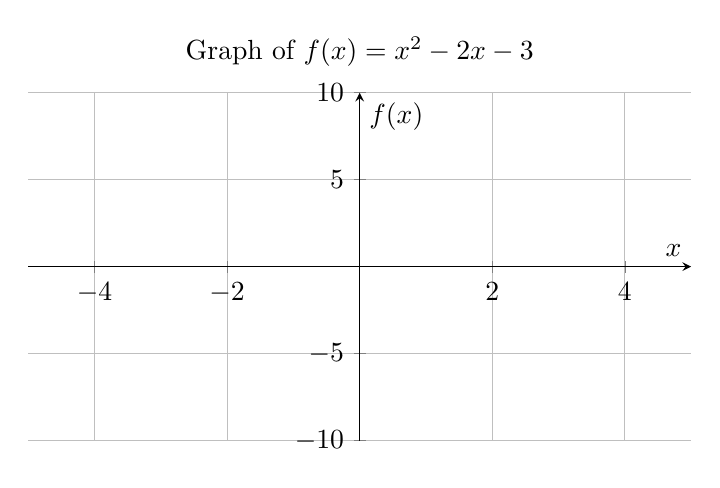
\begin{tikzpicture}
            \begin{axis}[
                axis lines = middle,
                xlabel = \(x\),
                ylabel = {\(f(x)\)},
                ymin=-10, ymax=10,
                xmin=-5, xmax=5,
                grid = major,
                width=10cm,
                height=6cm,
                domain=-5:5,
                samples=100,
                title={Graph of \( f(x) = x^2 - 2x - 3 \)}
            ]
            \end{axis}
        \end{tikzpicture}
    \end{center}

    \item Graph the function \( f(x) = -x^2 + 4x - 4 \). Identify the vertex and the points where the graph crosses the x-axis and y-axis.
    \begin{center}
        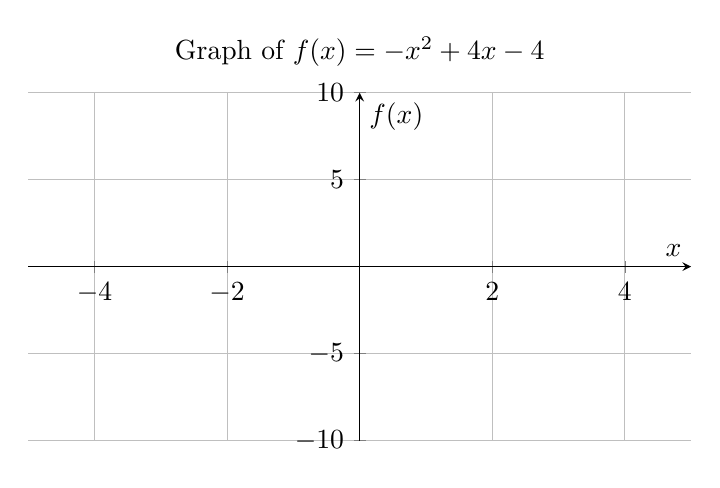
\begin{tikzpicture}
            \begin{axis}[
                axis lines = middle,
                xlabel = \(x\),
                ylabel = {\(f(x)\)},
                ymin=-10, ymax=10,
                xmin=-5, xmax=5,
                grid = major,
                width=10cm,
                height=6cm,
                domain=-5:5,
                samples=100,
                title={Graph of \( f(x) = -x^2 + 4x - 4 \)}
            ]
            \end{axis}
        \end{tikzpicture}
    \end{center}

    \item Graph the function \( f(x) = 2x^2 - 3x + 1 \). Identify the vertex and the points where the graph crosses the x-axis and y-axis.
    \begin{center}
        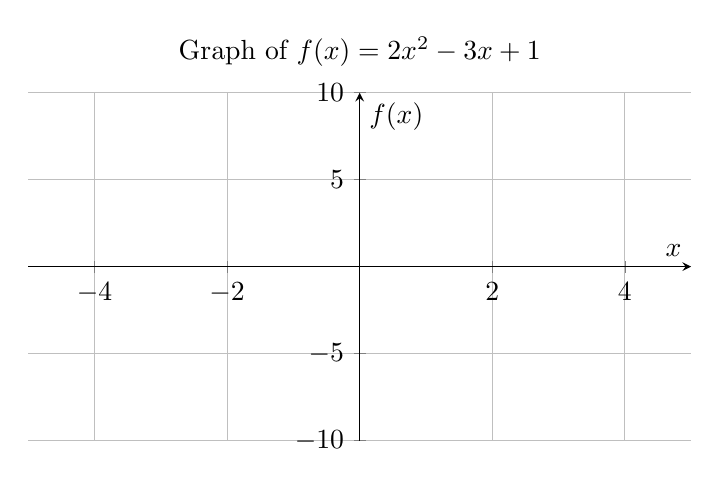
\begin{tikzpicture}
            \begin{axis}[
                axis lines = middle,
                xlabel = \(x\),
                ylabel = {\(f(x)\)},
                ymin=-10, ymax=10,
                xmin=-5, xmax=5,
                grid = major,
                width=10cm,
                height=6cm,
                domain=-5:5,
                samples=100,
                title={Graph of \( f(x) = 2x^2 - 3x + 1 \)}
            ]
            \end{axis}
        \end{tikzpicture}
    \end{center}

    \item Graph the function \( f(x) = -2x^2 + 5x - 3 \). Identify the vertex and the points where the graph crosses the x-axis and y-axis.
    \begin{center}
        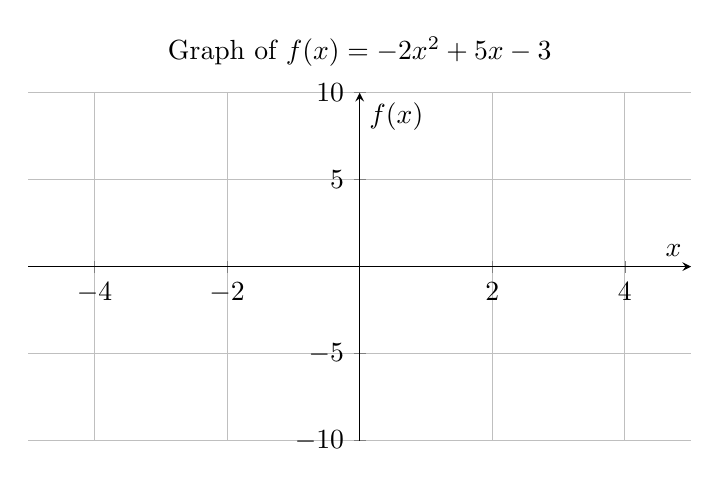
\begin{tikzpicture}
            \begin{axis}[
                axis lines = middle,
                xlabel = \(x\),
                ylabel = {\(f(x)\)},
                ymin=-10, ymax=10,
                xmin=-5, xmax=5,
                grid = major,
                width=10cm,
                height=6cm,
                domain=-5:5,
                samples=100,
                title={Graph of \( f(x) = -2x^2 + 5x - 3 \)}
            ]
            \end{axis}
        \end{tikzpicture}
    \end{center}

    \item Graph the function \( f(x) = x^2 + 4x + 4 \). Identify the vertex and the points where the graph crosses the x-axis and y-axis.
    \begin{center}
        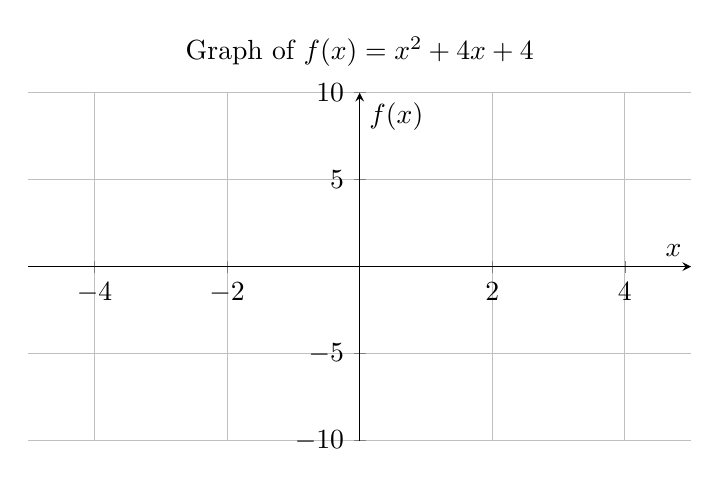
\begin{tikzpicture}
            \begin{axis}[
                axis lines = middle,
                xlabel = \(x\),
                ylabel = {\(f(x)\)},
                ymin=-10, ymax=10,
                xmin=-5, xmax=5,
                grid = major,
                width=10cm,
                height=6cm,
                domain=-5:5,
                samples=100,
                title={Graph of \( f(x) = x^2 + 4x + 4 \)}
            ]
            \end{axis}
        \end{tikzpicture}
    \end{center}

    \item Graph the function \( f(x) = -x^2 - 2x + 3 \). Identify the vertex and the points where the graph crosses the x-axis and y-axis.
    \begin{center}
        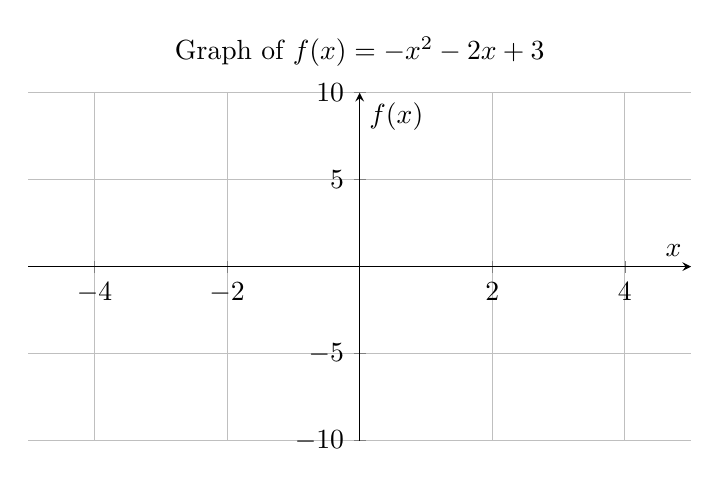
\begin{tikzpicture}
            \begin{axis}[
                axis lines = middle,
                xlabel = \(x\),
                ylabel = {\(f(x)\)},
                ymin=-10, ymax=10,
                xmin=-5, xmax=5,
                grid = major,
                width=10cm,
                height=6cm,
                domain=-5:5,
                samples=100,
                title={Graph of \( f(x) = -x^2 - 2x + 3 \)}
            ]
            \end{axis}
        \end{tikzpicture}
    \end{center}

    \item Graph the function \( f(x) = 3x^2 - 6x + 2 \). Identify the vertex and the points where the graph crosses the x-axis and y-axis.
    \begin{center}
        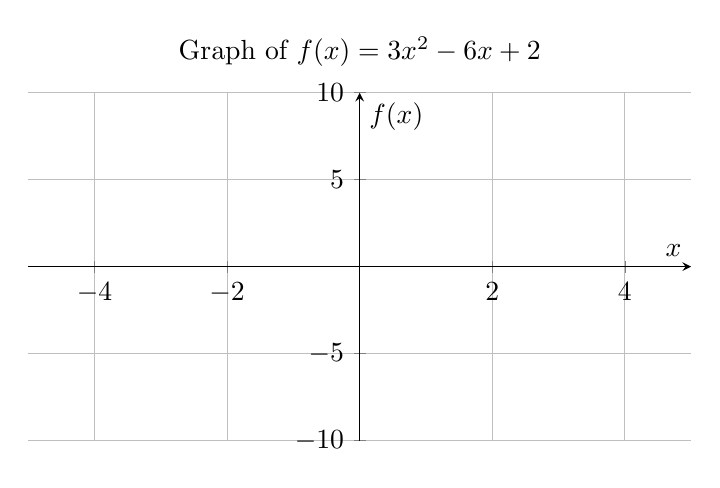
\begin{tikzpicture}
            \begin{axis}[
                axis lines = middle,
                xlabel = \(x\),
                ylabel = {\(f(x)\)},
                ymin=-10, ymax=10,
                xmin=-5, xmax=5,
                grid = major,
                width=10cm,
                height=6cm,
                domain=-5:5,
                samples=100,
                title={Graph of \( f(x) = 3x^2 - 6x + 2 \)}
            ]
            \end{axis}
        \end{tikzpicture}
    \end{center}

    \item Graph the function \( f(x) = -3x^2 + 2x + 1 \). Identify the vertex and the points where the graph crosses the x-axis and y-axis.
    \begin{center}
        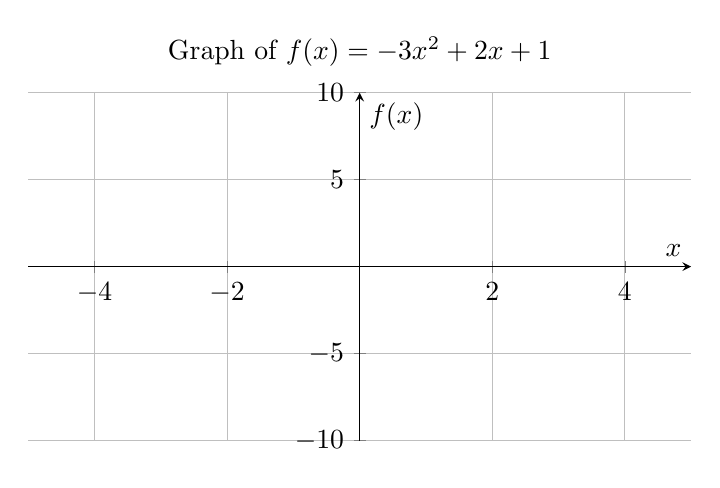
\begin{tikzpicture}
            \begin{axis}[
                axis lines = middle,
                xlabel = \(x\),
                ylabel = {\(f(x)\)},
                ymin=-10, ymax=10,
                xmin=-5, xmax=5,
                grid = major,
                width=10cm,
                height=6cm,
                domain=-5:5,
                samples=100,
                title={Graph of \( f(x) = -3x^2 + 2x + 1 \)}
            ]
            \end{axis}
        \end{tikzpicture}
    \end{center}

    \item Graph the function \( f(x) = x^2 - 6x + 9 \). Identify the vertex and the points where the graph crosses the x-axis and y-axis.
    \begin{center}
        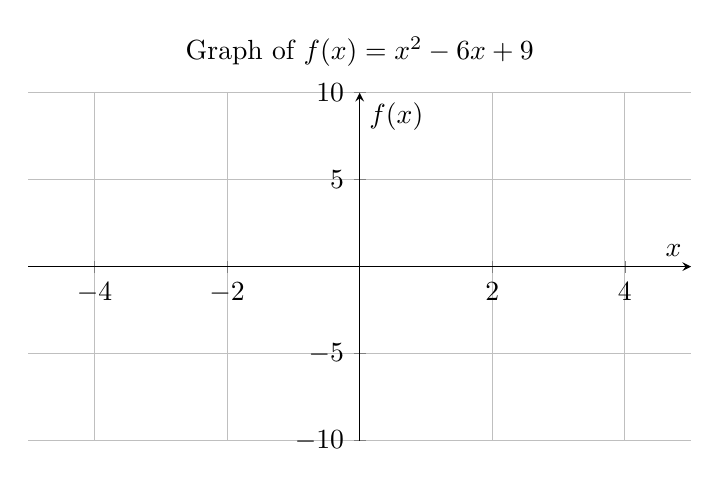
\begin{tikzpicture}
            \begin{axis}[
                axis lines = middle,
                xlabel = \(x\),
                ylabel = {\(f(x)\)},
                ymin=-10, ymax=10,
                xmin=-5, xmax=5,
                grid = major,
                width=10cm,
                height=6cm,
                domain=-5:5,
                samples=100,
                title={Graph of \( f(x) = x^2 - 6x + 9 \)}
            ]
            \end{axis}
        \end{tikzpicture}
    \end{center}

    \item Graph the function \( f(x) = -x^2 + 3x - 2 \). Identify the vertex and the points where the graph crosses the x-axis and y-axis.
    \begin{center}
        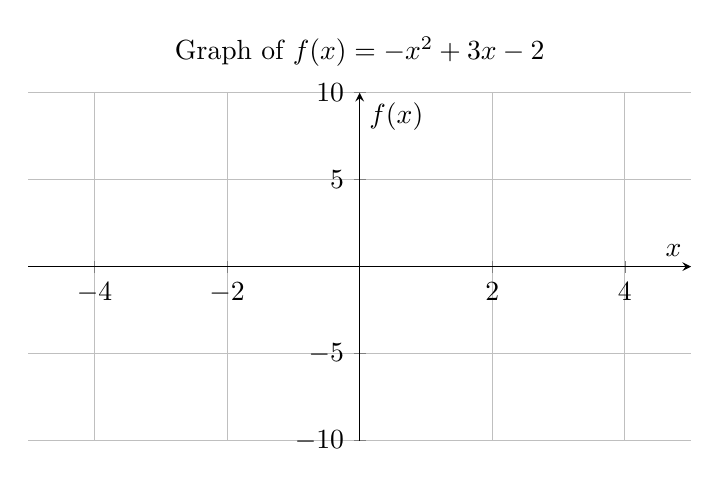
\begin{tikzpicture}
            \begin{axis}[
                axis lines = middle,
                xlabel = \(x\),
                ylabel = {\(f(x)\)},
                ymin=-10, ymax=10,
                xmin=-5, xmax=5,
                grid = major,
                width=10cm,
                height=6cm,
                domain=-5:5,
                samples=100,
                title={Graph of \( f(x) = -x^2 + 3x - 2 \)}
            ]
            \end{axis}
        \end{tikzpicture}
    \end{center}
\end{enumerate}
